\documentclass[a4paper,14pt,russian]{article}

\usepackage{extsizes}
\usepackage{cmap} % для кодировки шрифтов в pdf
\usepackage[utf8x]{inputenc}
\usepackage[russian]{babel}
\usepackage[T1,T2A]{fontenc}

\usepackage{algorithm}
\usepackage{algpseudocode}

\usepackage{graphicx} % для вставки картинок
\usepackage{epstopdf}

\usepackage{amssymb,amsfonts,amsmath,amsthm} % математические дополнения от АМС
% \usepackage[amsmath,thmmarks]{ntheorem}
\usepackage{indentfirst} % отделять первую строку раздела абзацным отступом тоже
\usepackage[usenames,dvipsnames]{color} % названия цветов
\usepackage{makecell}
\usepackage{multirow} % улучшенное форматирование таблиц

\usepackage{hyperref}
\usepackage{cleveref}
\usepackage{url}
% \usepackage[none]{hyphenat}

\usepackage{geometry}
\geometry{left=3cm}
\geometry{right=1cm}
\geometry{top=2cm}
\geometry{bottom=3cm}
% \usepackage{babel}
\tolerance=1
\emergencystretch=\maxdimen
\hyphenpenalty=10000
\hbadness=10000



\linespread{1.3} % полуторный интервал
% \renewcommand{\rmdefault}{ftm} % Times New Roman
% \frenchspacing

% ituphanov
% Надо разобраться с полями. Сейчас диплом выглядит как книжка-малышка.

% \usepackage{fancyhdr}
% \pagestyle{fancy}
% \fancyhf{}
% \fancyfoot[C]{\normalsize \thepage}
% \fancyheadoffset{0mm}
% \fancyfootoffset{0mm}
% \setlength{\headheight}{17pt}
% \renewcommand{\headrulewidth}{0pt}
% \renewcommand{\footrulewidth}{0pt}
% \fancypagestyle{plain}{
%     \fancyhf{}
%     \rhead{\thepage}}

\pagenumbering{arabic}

\setcounter{page}{2}

\usepackage[tableposition=top]{caption}
\usepackage{subcaption}
\DeclareCaptionLabelFormat{gostfigure}{Рисунок #2}
\DeclareCaptionLabelFormat{gosttable}{Таблица #2}
\DeclareCaptionLabelSeparator{gost}{~---~}
\captionsetup{labelsep=gost}
\captionsetup[figure]{labelformat=gostfigure}
\captionsetup[table]{labelformat=gosttable}
\renewcommand{\thesubfigure}{\asbuk{subfigure}}


\begin{document}
\tableofcontents
\newpage

\section*{Аннотация}

В работе описывается программа для построения оптимального плана выполнения заданий несколькими подводными аппаратами. Работа выполнена в рамках системы управления АНПА для подводных аппаратов ДВФУ. Рассмотрен ряд алгоритмов для реализации такого построения. Проведено их тестирование на сгенерированных и составленных в ручную тестах, после чего наиболее эффективные алгоритмы для различных размеров входных данных внедрены в систему управления.

\section{Введение}
\subsection{Глоссарий}
\begin{itemize}
\item АНПА -- Автономный необитаемый подводный аппарат \cite{auv}.
\item СПУ -- Система программного управления.
\item MTSP -- Multiple Traveling Salesman Problem или множественная задача коммивояжера \cite{bektas2006multiple}.
\item ГА -- генетический алгоритм \cite{ga}.
\end{itemize}

\subsection{Описание предметной области}

Одна из областей применения автономных необитаемых подводных аппаратов заключается в решении обзорно-поисковых задач. В рамках таких задач аппаратами покрывается некоторая площадь под водой с целью, например, построения карты с нанесенными результатами измерений, либо с целью поиска и обследования заданных объектов.

В настоящее время ведутся исследования методов, которые позволят более эффективно решать обзорно-поисковые задачи за счет интеллектуализации аппаратов.
Например, в работе \cite{cannell2006boundary} описывается алгоритм использования автономного необитаемого водного аппарата (АНВА) для обнаружения шлейфов теплой воды с атомной электростанции в морской среде.

Все больше методов концентрируются на эффективном использовании группы АНПА для решения подобных задач.
Так, в работе \cite{purcell2011use} описывается случай успешного использования автономных подводных аппаратов для обнаружения авиалайнера, потерпевшего крушение в водах Атлантического океана, спустя год после происшествия. Для поиска затонувшего объекта использовались АНПА REMUS 6000 \cite{sharp2008more}.

В России исследования по разработке более эффективных методов решения обзорно-поисковых задач с использованием подводных аппаратов ведутся в том числе ИПМТ ДВО РАН и ДВФУ. Некоторые исследования методов, основанных на централизованном управлении группой АНПА, описаны в работах \cite{tuphanov1} и \cite{tuphanov2}. В этих работах аппараты используются для обследования локальных неоднородностей морской среды.

Подбронее о современных аппаратах, производимых серийно, и задачах, которые они решают, можно узнать в работе \cite{auvs}.

Одиним из основных подводных аппаратов ДВФУ, предназначенных для исследований групповой работы АНПА, является аппарат МАРК (морской автономный робототехнический комплекс) \cite{marc}.

\subsection{Неформальная постановка задачи}

% описание конкретных предметных областей, примеры использования
% Часть взять из формальной постановке
% планирование в реальном времени, порядок величины миссии
% Перепланирование из-за различных сбоев или добавлений новых аппаратов
% время наработки на отказ
% батарея
% упоминание конкретных аппаратов
% Перепланирование по причине изменения входных данных (добавление-удаление аппаратов, изменение заданий, причины этого, добавление, удаление заданий)
% Почему модель учитывает некоторые факторы а некоторые - нет
% Время поворота, размеры лодок, реальные планы, карты
% Как покрываем площади?
% Почему решаем такую общую задачу.
% Почему разбиваем задачу на две (составление заданий и распределения), а не составляем сразу оптимальные траектории
% Предполагаем
% Улучшить в рамках существующей системы

В настоящее время в ДВФУ организация работы группы аппаратов осуществляется следующим образом:
\begin{enumerate}
\item Заранее составляются задания для аппаратов. Отдельное задание может заключаться в прохождении от одной точки подводной среды к другой с заданной скоростью, возможно, с заданной траекторией, с целью съемки дна гидролокатором, замера параметров водной среды и т.п.
\item Далее, система управления аппаратами, запущенная с настольного ПК или ноутбука, определяет множество аппаратов, между которыми необходимо оптимальным образом распределить вышеописанные задания.
\item Затем СПУ запускает алгоритм-планировщик для поиска оптимального распределения заданий между аппаратами. Этот алгоритм для каждого аппарата определит план (последовательность заданий), который аппарату необходимо выполнить. Каждое задание может выполнять только один аппарат, единственный раз.
\item Индивидуальные планы рассылаются аппаратам по сети, после чего начинается их выполнение.
\end{enumerate}

Во время выполнения планов могут возникать непредвиденные ситуации, такие как:
\begin{itemize}
\item Появление нового аппарата, готового к выполнению заданий
\item Выход аппарата из строя. Это может произойти как по причине поломки, так и ввиду того, что все аппараты используют батареи для электропитания, которые разряжаются в течение нескольких часов.
\item Могут появиться новые задания, по причине, например, обнаружения аппаратами новых областей для обследования.
\item Существующие задания могут измениться. Может измениться время, которое аппарату необходимо потратить на выполнение задания, могут измениться начальные и конечные точки в виду, например, помех из-за появления новых объектов в морской акватории.
\end{itemize}

В случае возникновения любой из вышеперечисленных непредвиденных ситуаций, СПУ составляет план заново, учитывая занятость аппаратами выполнением заданий, которые нельзя прерывать, и принимая во внимания изменившиеся данные для планирования. Обновленные планы аппаратов рассылаются по сети. Каждый аппарат начинает выполнять новый план по завершению последнего задания, в котором был задействован.

В существующей СПУ используется алгоритм поиска оптимального плана.
Временная сложность данного алгоритма экспоненциально зависит от количества заданий, по этой причине он работает слишком долго, если количество заданий превышает 20. % у меня на ноуте по крайней мере для 20 заданий и двух аппаратов я за пару минут его не дождался
В следствии этого лабораторией необитаемых подводных аппаратов и их систем в ДВФУ была предложена задача, разработать и исследовать новые алгоритмы планирования заданий между группой АНПА с целью их последующего внедрения в систему управления.

\subsection{Обзор существующих решений} \label{mtsp-graph}

Существует большое множество алгоритмов, использующихся для решения задачи централизованного планирования заданий для группы аппаратов.
Все найденные подходы используют алгоритмы решения известной задачи дискретной оптимизации, MTSP, в разных ее вариантах.
В такой задаче каждому заданию соответствует единственная точка пространства, которую необходимо посетить единственный раз, только одному аппарату.

Один из вариантов постановки задачи MTSP выглядит следующим образом:
\begin{itemize}
\item Имеется граф $G(V, E)$.
\item $V = {v_0, v_1, ... , v_n}$ -- множество вершин ($v_0$ - единственная стартовая позиция всех аппаратов, $v_1, ..., v_n$ -- координаты точек-заданий).
\item $E$ -- множество ребер $\{(v_i, v_j) | i \neq j\}$. Каждое ребро $(v_i, v_j)$ означает наличие перехода от задания $v_i$ к заданию $v_j$. Применительно к подводным аппаратам граф $G$, как правило, является полным.
\item $C$ -- матрица весов $c_{i j}$ каждого ребра (стоимость перехода между заданиями).
\item $R_k$ -- маршрут $k$-го аппарата, $k=1..m$ (неразрывная последовательность ребер).
\item $\widetilde{C}(R_k) = \displaystyle\sum_{(v_i, v_j) \in R_k} c_{i j}$ -- стоимость маршрута $R_k \subseteq E$.
\end{itemize}
Задача состоит в определении такого множества из $m$ маршрутов, что наибольшая стоимость маршрута является минимально возможной:
\begin{equation} \label{mtsp1}
\displaystyle \max_{k=1..m} \widetilde{C}(R_k) \rightarrow \min
\end{equation}

В других вариантах может меняться оптимизируемый функционал, стартовых позиций может быть несколько, и так далее. Подробнее о данной задаче и о методах ее решения можно узнать в работе \cite{bektas2006multiple}.
В частности, в \cite{binaryprog} описан метод, основанный на применении целочисленного программирования к решению MTSP с различными исходными положениями аппаратов.

Однако, большинство подходов находят приближенное решение множественной задачи коммивояжера, так как точные алгоритмы работают медленно. В работе \cite{kiraly2010novel} к решению MTSP применен генетический алгоритм, а в \cite{na2007heurisic} описаны эвристические методы распределения заданий между аппаратами с последующим решением задачи коммивояжера для каждого из них в отдельности.

В ДВФУ для решения задачи планирования используют решение, описанное в работе \cite{tuphanov1}. Данное решение является точным в рамках используемой модели, но работает слишком медленно для необходимого количество заданий и аппаратов. В связи с этим необходимо исследование других подходов к задаче группового управления.

Для постановки задачи оптимизации заказчик использует новую модель, в рамках которой и работает вышеупомянутое решение. Она также описана в работе \cite{tuphanov1}. Ни один из найденных методов ее не рассматривает, поэтому некоторые из них решено было доработать для решения задачи в рамках новой модели.

\section{Математические методы}

\subsection{Постановка задачи}
В данном разделе описывается модель, использующаяся для решения задачи планирования в СПУ заказчика.

Предполагается, что имеется $m$ аппаратов и $n$ заданий. Планирование происходит перед началом миссии. Известно, что $q$-ый аппарат в начальный момент времени находится в точке $\mathbf{s_q}$ и готов к выполнению заданий. Вводится функция $d_q(\mathbf{a}, \mathbf{b})$, обозначающая время перехода АНПА от точки $\mathbf{a}$ к точке $\mathbf{b}$. Она принимает вид $d_q(\mathbf{a}, \mathbf{b}) = |\mathbf{a} - \mathbf{b}| / u_q$, где $u_q$ - максимальная скорость $q$-го аппарата. Для $i$-го задания дано $v_i$ вариантов его выполнения и $j$-ый вариант характеризуется тройкой $(\mathbf{a}_{i  j}, \mathbf{b}_{i j}, l_{i j})$, обозначающей соответственно точку начала задания, точку окончания и время его выполнения.

Время выполнения $l_{i j}$ может зависеть как от координат $\mathbf{a}_{i j}$ и $\mathbf{b}_{i j}$, так и от других параметров. Алгоритм решения задачи планирования никак не учитывает зависимости $l_{i j}$ от каких-либо параметров, предполагается, что эти величины известны на этапе составления заданий и будут даны на вход алгоритму.

Планом аппарата названа последовательность пар \\ $p = ((i_1, j_1), (i_2, j_2), ..., (i_{|p|}, j_{|p|}))$ такая, что $i_k \in 1..n, j_k \in 1..v_{i_k}$, для всех $k \in 1..|p|$. Выполнение плана $q$-м аппаратом начинается в точке $\mathbf{s}_q$ и заканчивается в точке $\mathbf{b}_{i_{|p|} j_{|p|}}$. Время выполнения аппаратом с номером $q$ плана $p$, составляет:

\begin{equation} \label{varm1}
t_q(p_q) = d_q(\mathbf{s}_q, \mathbf{a}_{i_1 j_1}) + \sum_{k=2}^{|p|} d_q(\mathbf{b}_{i_{k-1} j_{k - 1}}, \mathbf{a}_{i_k j_k}) + \sum_{k=1}^{|p|}l_{i_k j_k}
\end{equation}

Общим планом является кортеж планов $P = (p_1, p_2, ..., p_m)$ такой, что каждое здание встречается среди его планов один раз и в одном варианте. $|P| = m$ (количество планов совпадает с количеством аппаратов). Время выполнения общего плана определяется выражением:

\begin{equation} \label{varm2}
t(P) = \displaystyle \max_{q \in 1..m} t_q(p_q)
\end{equation}

Задача состоит в том, чтобы при данных стартовых позициях $\mathbf{s}_q$, известных заданиях и вариантах их выполнения найти общий план $P$, минимизирующий $t(P)$:
\begin{equation} \label{varm3}
t(P) \rightarrow \min
\end{equation}


\subsection{Алгоритмы}
\subsubsection{Целочисленное программирование}

В настоящем разделе описывается алгоритм нахождения точного решения к поставленной задаче с помощью методов целочисленного программирования.

Целочисленное программирование является весьма популярным подходом для поиска точного решения в задаче коммивояжера.
Программный пакет Concorde, основанный на данном подходе, за несколько секунд решает задачу 1го коммивояжера для сотен городов \cite{applegate1999concorde}.
Поэтому было решено воспользоваться данным методом для задачи планирования. Однако, в сравнении с основной моделью \eqref{varm1}~--~\eqref{varm3} был сделан ряд упрощений:

\begin{itemize}
\item Все задания имеют ровно один вариант выполнения.
\item У каждого задания начальная и конечная точки совпадают.
\item Временные затраты на выполнение самих заданий аппаратами пренебрежимо малы.
\item Скорости аппаратов одинаковы.
\item Аппараты в начальный момент времени готовы к выполнению миссии.
\item Для описания координат аппаратов и заданий используется двумерная декартова система координат.
\end{itemize}
Данные упрощения были сделаны для сведения задачи к MTSP \eqref{mtsp1}.


\paragraph{Сведение исходной задачи к MTSP} ~\\

Введем ориентированный граф $G(V, E)$ аналогично \eqref{mtsp-graph}. И рассмотрим задачу оптимизации \eqref{mtsp1}.
В нашем случае множество вершин состоит из $m$ стартовых позиций аппаратов и $n$ заданий. Из всех стартовых позиций существуют переходы к заданиям. Существуют также переходы между любыми двумя различными заданиями. Для сохранения задачи в варианте \eqref{mtsp1} при различных стартовых позициях, необходимо также ввести фиктивную вершину $v_0$, из которой проведены ребра к стартовым позициям и в которую ведут ребра из каждого задания:
\begin{align*}
& E = \{(v_0, v_j)|j = 1..m\} \cup \\
& \cup \{(v_i, v_0) | i = m+1..m+n\} \cup  \\
& \cup \{(v_i, v_j)| i \neq j; i,j=m+1..m+n\} \cup \\
& \cup \{(v_i, v_j)| i = 1..m, j = m+1..m+n\}
\end{align*}

Весом каждого ребра будет расстояние между координатами точек, соответствующих вершинам. Вес ребер, инцидентных, фиктивной вершине равен нулю.
На построенном графе необходимо решить задачу \eqref{mtsp1}.

% ituphanov (3): Если бы ты писал книгу (или статью), то несколько предыдущих абзацев точно
% надо было бы переделать. Потому что ты объяснил на пальцах и можно как-то не так это понять.
% Потому что встречаются словосочетания "вершина аппарата", и когда пытаешься понять что это
% такое, то видишь "стартовая вершина аппарата". При этом может создаться впечатление, что
% ты путаешь вершины графа и точки на плоскости (хотя, мы оба знаем, что не путаешь).
% Более правильным был бы способ описания, где ты ввёл бы обозначения для графа G, множества
% рёбер E, множества вершин V, подмножеств множества V, отвечающих за разные вещи,
% фиктивной вершины и т.д. и описал бы весовую функцию его рёбер. Какие-то из рёбер весят 0,
% какие-то - бесконечность, а какие-то ровно столько, каково расстояние между соответствующими
% точками на плоскости. Вершины можно также занумеровать (как ты это сделал ниже).
% Тогда можно нарисовать красивую матрицу для весовой функции, и использовать введённые
% обозначения ниже при описании задачи ЛП.
% Хорошо бы всё это сделать, если будет время.

% Вставить пример графа.


\paragraph{Постановка задачи целочисленного программирования} ~\\

Вводим бинарные переменные $x_{i j k}$, где $i, j = 0..m+n$ -- номера вершин графа $G$, $k = 1..m$ -- номер аппарата. Полагаем $x_{i j k}$ равным единице, если в цикле, соответствующему аппарату $k$, есть ребро $(v_i, v_j)$, и нулю -- в противоположном случае.

% ituphanov
% векторов размерности $n (m+n+1)^2$ - здесь, вроде n на m надо заменить.
$\mathbf{x} \in \{0,1\}^{m (m+n+1)^2}$ ~-- пространство всех бинарных векторов размерности $n (m+n+1)^2$. $\mathbf{x} = (x_{0, 0, 0}, ..., x_{m+n, m+n, m})$.

Добавляем следующие ограничения:
\begin{itemize}

\item Каждый аппарат должен иметь у себя в цикле ровно одно ребро, входящее в фиктивную вершину и выходящее из нее:

\begin{equation} \label{lin1}
 \displaystyle\sum_j x_{0 j k} = \displaystyle\sum_i x_{i 0 k} = 1, ~k = 1..m
\end{equation}

\item Сумма ребер, выходящих из любой вершины, кроме фиктивной, должна быть равна сумме ребер, входящих в нее и равна единице:
\begin{equation}
\displaystyle\sum_j \displaystyle\sum_k x_{i j k} = \displaystyle\sum_j \displaystyle\sum_k x_{j i k} = 1, ~\forall i \neq 0
\end{equation}

\end{itemize}

Обозначим вес ребра $(i, j)$ как $w_{i j}$. Тогда стоимость маршрута каждого аппарата:
\begin{equation}
c_k(\mathbf{x}) = \displaystyle\sum_i \displaystyle\sum_j w_{i j} x_{i j k}, ~\mathbf{x} = \{x_{i j k} | i, j = 0..m+n, k = 1..m\}
\end{equation}


\begin{itemize}
\item В первом варианте алгоритма минимизируемым функционалом является
\begin{equation}
\widetilde{c}(\mathbf{x}) = \displaystyle\max_k \{c_k(\mathbf{x})\}
\end{equation}

\item Во втором варианте мы вводим переменную $C_{max}$, оптимальное значение котоорой ищем бинарным поиском. На каждой итерации бинарного поиска проверяем существование решения задачи целочисленного программирования, в которую добавлены ограничения $c_k(\mathbf{x}) \le C_{max}$ и минимизируемым функционалом является сумма:
\begin{equation}
\widetilde{c}(\mathbf{x}) = \displaystyle\sum_k c_k(\mathbf{x})
\end{equation}

\begin{equation} \label{lin2}
\widetilde{c}(\mathbf{x}) \rightarrow \min
\end{equation}

\end{itemize}


\paragraph{Неравенства циклов} ~\\

При вышеописанной постановке задачи целочисленного программирования мы легко можем получить в качестве решения не один, а систему циклов для одного или нескольких аппаратов. Чтобы этого избежать, необходимо вводить дополнительные линейные ограничения исключающие появление систем циклов. В данной работе использовался следующий метод:
\begin{enumerate}
\item  Ожидаем решения задачи целочисленного программирования.
\item Анализируем решение на наличие систем циклов. Для этого используем поиск в глубину для каждого аппарата.
\item Если поиск в глубину находит цикл, длина которого меньше суммарного количества ребер, задействованных данным аппаратом, значит у данного аппарата в маршруте есть несколько циклов.
\item Пусть $k$ ~-- аппарат, у которого найден вышеописанный цикл, $A$ ~-- множество пар $(i, j)$ таких, что ребро $(i, j)$ является частью цикла. Тогда для данного аппарата добавляем к задаче \eqref{lin1}~--~\eqref{lin2} следующее линейное ограничение:
\begin{equation} \label{lin3}
\displaystyle \sum_{(i,j) \in A} x_{i j k} \le |A| - 1
\end{equation}

\item Решаем задачу \eqref{lin1}~--~\eqref{lin3}, переходим к шагу 1.
\end{enumerate}

Аналогичные условия для исключения циклов использовались, например, в работе \cite{shmoys1990analyzing}.

\paragraph{Реализация} ~\\
Решением линейной задачи оптимизации (\eqref{lin1}~--~\eqref{lin3}) являются значения переменных  $x_{i j k}$, доставляющие максимум в целевой функционал \eqref{lin2}.
Значение этих переменных могут вовсе не быть целыми, хотя мы предполагаем, что $x_{i j k}$ принимают только целые значения $0$ или $1$. Данную проблему решает метод ветвей и границ, позволяющий решать линейные задачи оптимизации в целых числах. Этот метод давно известен (о нем можно прочитать в работе \cite{lawler1966branch}) и реализован в различных библиотеках для языка программирования C++.
В данной работе использовался фреймверк SYMPHONY \cite{ralphs2005symphony}, реализующий данный метод.
Для формулировки задачи целочисленного программирования на языке программирования C++ использовался фреймверк FlopCpp \cite{hultberg2007flopc++}.

\subsubsection{Жадный алгоритм}
% Почему такой жадник
Жадный алгоритм действует следующим образом:
\begin{enumerate}
\item Переберем все задания и их варианты.
\item Каждый вариант задания попытаемся вставить в план каждому аппарату.
\item Выберем тот аппарат, после вставки данного варианта задания которому, время выполнения его плана будет наименьшим.
\item Вставим это задание выбранному аппарату в план, в наиболее подходящее место.
\item После вставки методом динамического программирования определим оптимальные варианты всех заданий в плане выбранного аппарата.
\end{enumerate}

\pagebreak

\begin{algorithm}
\floatname{algorithm}{Алгоритм}
\caption{Жадный алгоритм}\label{alg:greedy}
\begin{algorithmic}[1]

\ForAll {$t \in T$}
    \ForAll {$var \in Vars(t)$}
        \ForAll {$v \in V$}
            \State $time, pos \gets$ \Call{MinPathTime}{$t, var, Plan(v)}$
            \If {$time < minTime$}
                \State $minTime \gets time$
                \State $bestPos \gets pos$
                \State $bestV \gets v$
                \State $bestVar \gets var$
            \EndIf
        \EndFor
    \EndFor
    \State \Call{Insert}{$t, bestVar, Plan(bestV), bestPos$}
    \State \Call{OptimizeVars}{$bestV$}
\EndFor

\end{algorithmic}
\end{algorithm}

Функция $OptimizeVars$ в данном алгоритме устанавливает оптимальные варианты заданий в плане аппарата $bestV$ с помощью метода динамического программирования по двум измерениям: номер последнего задания в последовательности и номер варианта. Эта функция устроена следующим образом:

\pagebreak

\begin{algorithm}
\floatname{algorithm}{Алгоритм}
\caption{Оптимальный выбор вариантов}\label{alg:dynamic}
\begin{algorithmic}[1]
\Procedure{OptimizeVars}{v}
    \State $p \gets Plan(v)$
    \State $k \gets 0$
    \For {$i \in Vars(First(p))$}
        \State $d[0][i] \gets DistFromStart(First(p))$
    \EndFor
    \For {$i = 1..Size(p)$}
        \ForAll{$var1 \in Vars(p[i - 1])$}
            \ForAll{$var2 \in Vars(p[i])$}
                \State $val \gets d[i - 1][var1] + Dist(p[i - 1], var1, p[i], var2)$
                \If {$d[i][var2] > val$}
                    \State $d[i][var2] \gets Min(d[i][var2], val)$
                    \State $prev[i][var2] \gets var1$
                \EndIf
            \EndFor
        \EndFor
    \EndFor
    \State \Call{SetNewVars}{$p, d, prev$}
\EndProcedure
\end{algorithmic}
\end{algorithm}

Если считать количество заданий константным, асимптотика времени работы жадного алгоритма ~-- $O(n^2)$, где $n$ ~-- количество заданий.


\subsubsection{Генетический алгоритм}
Генетические алгоритмы часто используют в задачах коммивояжера и, соответственно, задачах планирования заданий для групп роботов. ГА используются для нахождения приближенного решения задачи, однако, их преимущество в том, что работают они гораздо быстрее точных алгоритмов.

В качестве параметров ГА использовались:
\begin{itemize}
\item Количество итераций $n$.
\item Размер популяции $s$.
\item Вероятность мутации $p_m$.
\item Процент выживших особей в популяции $p_a$. Для данного ГА была использована стратегия элитарности, когда лучшие особи в поколение не погибают.
\end{itemize}

Генетический алгоритм начинается генерацией случайной популяции.
Далее выполняются $s$ итераций алгоритма, после чего, независимо от качества полученного решения, алгоритм завершается.
Каждая итерация алгоритма работает следующим образом:
\begin{enumerate}
\item Каждая особь мутирует с вероятностью $p_m$.
\item Согласно проценту выживших особей определяется количество $s_d$ погибающих особей.
\item Среди всех особей популяции равновероятно выбираются $s_d$ скрещивающихся пар.
\item Каждая скрещивающаяся пара производит две особи, из которых равновероятно выбирается одна выжившая.
\item Вычисляется функция приспособленности для каждой особи, после чего $p_a$ процентов особей остается в популяции, а остальные заменяются произведенным ранее потомством.
\end{enumerate}

\paragraph{Особи} ~\\
В статье \cite{kiraly2010novel} были рассмотрены несколько представлений решения в виде хромосом для множественной задачи коммивояжера. Согласно полученным в данной статье результатам, наиболее оптимальным было представление решения в виде двух хромосом:
\begin{enumerate}
\item Перестановка номеров заданий.
\item Последовательность номеров аппаратов, соответствующих номерам заданий в первой хромосоме.
\end{enumerate}

Данное представление было использовано и для решения задачи \eqref{varm1}~--~\eqref{varm3}. Однако для учета разных вариантов заданий, необходимо было ввести дополнительную хромосому -- номера вариантов заданий, соответствующих первой хромосоме.

\paragraph{Мутации} ~\\
Каждая особь с вероятностью $p_m$ может быть подвергнута трем видам мутаций.
\begin{enumerate}
\item В каждой хромосоме по очереди равновероятно выбираются две позиции, элементы между которыми устанавливаются в обратном порядке.
\item В каждой хромосоме по очереди равновероятно выбираются две позиции, элементы в которых меняются местами.
\item Во второй хромосоме равновероятно выбирается случайный элемент, значение в котором заменяется случайным номером аппарата.
\end{enumerate}


\paragraph{Скрещивание} ~\\
Первая хромосома каждой особи представлена в виде перестановки. Возникает проблема при скрещивании таких хромосом, ведь обычный обмен частями хромосом приводит к нарушению корректности перестановки. Существуют различные способы скрещивания перестановок. Среди них был выбран PMX (Partially Matched Crossover), о нем можно подробнее узнать в работе \cite{goldberg1985alleles}

\pagebreak
\begin{figure}[here]
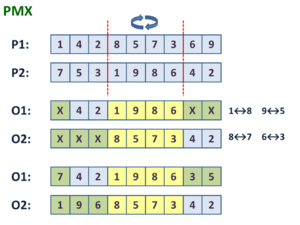
\includegraphics{images/300px-Pmx.png}
\caption{Partially matched crossover}
\label{fig:pmx}
\end{figure}

На \cref{fig:pmx} показан принцип работы оператора скрещивания.
\begin{enumerate}
\item Сначала равновероятно определяются две границы обмениваемой области хромосом. Такой обмен задает взаимно-однозначное преобразование между элементами перестановок.
\item Затем, воспользовавшись данным преобразованием, можно разрешить конфликты, возникающие в остальных областях скрещивающихся хромосом.
\end{enumerate}
Все хромосомы кроме первой в используемом алгоритме не скрещиваются.

\paragraph{Функция приспособленности} ~\\
Функция приспособленности предполагает, что задания в первой хромосоме должны быть внесены в план выполнения в порядке слева направо.
Далее, с помощью алгоритма \eqref{alg:dynamic}, немного измененного для работы с хромосомами, вычисляются оптимальные варианты заданий.
После чего вычисляется функционал \eqref{varm3} стоимости решения.


\section{Требования}


% Столкновения бывают но мы на них забиываем

Программа должна:
\begin{itemize}
\item Реализовывать и сравнивать несколько алгоритмов решения задачи планирования
\item Работать как часть системы программного управления для АНПА ДВФУ.
\end{itemize}

Лучшие из реализованных алгоритмов для различных размеров входных данных требуется внедрить в уже использующуся систему планирования заданий для подводных аппаратов ДВФУ, работающую под операционными системами семейства Linux. В результате внедрения новых алгоритмов система должна:
\begin{itemize}

\item Осуществлять планирование до 100 заданий для группы до 5 аппаратов за приемлемое время (до 1 минуты).
\item Выбирать более эффективный алгоритм в зависимости от размеров входных данных для планирования.
\item Допускается отклонение решения от оптимального на некоторых входных данных, в случае если алгоритм, дающий точное решение неэффективно на них работает.
\end{itemize}

\section{Проект}
\subsection{Объектно-ориентированная структура}
Система состоит из следующих модулей
\begin{itemize}
\item Task. Содержит классы:
    \begin{itemize}
    \item pnt. Содержит основной набор функций для работы с трехмерными векторами в евклидовом пространстве.
    \item assigned\_task. Содержит информацию об использованном варианте задания (начальная, конечная точки и время выполнения).
    \item task\_t. Содержит набор функций для работы с заданиями.
    \item tasks\_type. Контейнер для хранения заданий. Содержит функционал для добавления и доступа к заданиям.
    \end{itemize}
\item Solver. Содержит единственный класс basic\_solver, являющийся базовым ко всем классам, инкапсулирующим различные алгоритмы решения задачи планирования заданий для группы АНПА.
\item Plan. Содержит единственный класс plan\_t, который инкапсулирует работу с общим планом для всех аппаратов.
\item Data. Содержи тединственный класс problem\_data, содержащий входные данные к задаче (координаты начал и концов заданий, стартовые положения и максимальные скорости аппаратов) и предоставляющий к ним доступ.
\item Visualize. Содержит класс visual\_frame, который служит для вывода заданного общего плана для группы аппаратов на экран.
\item MILPSolver. Содержит класс milp\_solver, в котором находится реализация алгоритма, основанного на целочисленном программировании.
\item GreedySolver. Содержит класс greedy\_solver, реализующий жадный подход к решению задачи планирования.
\item GeneticSolver. Содержит класс genetic\_solver, реализующий генетический алгоритм для решения исходной задачи.
\item HKSolver. Содержит класс, содержащий реализацию алгоритма, описанного в \cite{tuphanov1}
\end{itemize}

На \cref{fig:modules} показаны зависимости между модулями программы.

\pagebreak
\begin{figure}[here]
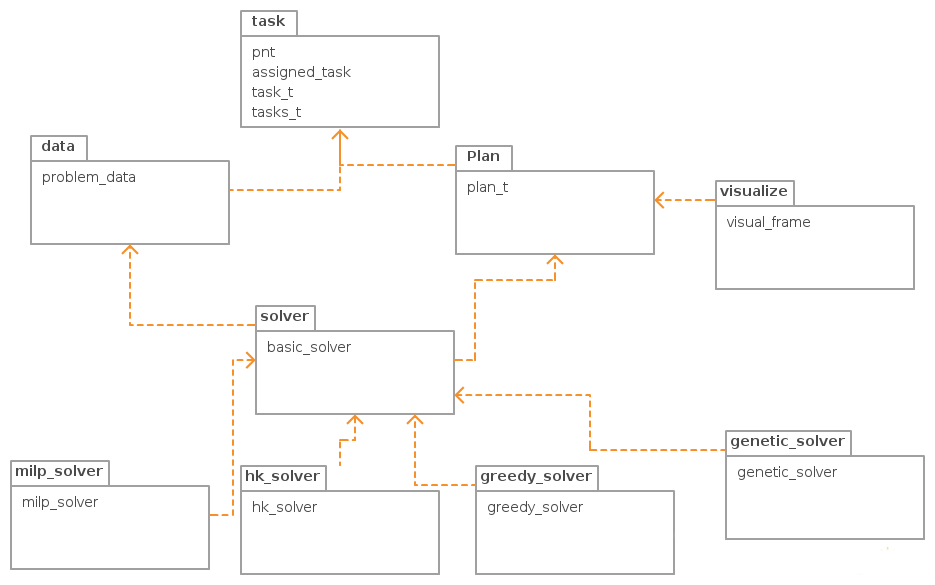
\includegraphics[scale=0.5]{images/group-control.png}
\caption{Модули системы}
\label{fig:modules}
\end{figure}

\section{Тестирование}
Для оценки качества работы алгоритмов была использована визуализация решений с помощью библиотеки OpenCV \cite{bradski2008learning}.
Кроме того была написана утилита с интерфейсом командной строки на языке Python, которая может запускать разные алгоритмы на различных тестах, сохранять полученные решения в формате csv, а затем визуализировать величину полученного решения для каждого алгоритма в зависимости от номера теста.
Для реализации использовались библиотеки pandas \cite{mckinney2010data} и matplotlib \cite{hunter2007matplotlib}. Генетический алгоритм запускался с параметрами:
\begin{enumerate}
\item Размер популяции $s = 1000$
\item Вероятность мутации $p_m = 0.15$
\item 20\% лучших особей в популяции выживают
\item Количество итераций $n = 2000$
\end{enumerate}

Асимптотика времени работы одной итерации ГА ~-- $O(s n + s\log(s))$
При такой конфигурации ГА работал на всех тестах от 30 до 60 секунд.

Были получены следующие результаты.

\begin{figure}[here]
\includegraphics[scale=0.6]{images/test_small1.jpg}
\caption{Зависимость стоимости решения от номера теста для всех алгоритмов. 2 аппарата, до 18 заданий.}
\label{fig:alg_small}
\end{figure}
% \pagebreak

На \cref{fig:alg_small} показаны результаты запуска алгоритмов на тестах с 2мя аппаратами и до 18 заданий. Точное решение (hk\_solver) на них работает не более 10 секунд. Видно, что на таких размерах входных данных выгоднее использовать именно его. Также можно заметить, что генетический алгоритм находит приближенное решение гораздо более близкое к точному, чем жадное.

\begin{figure}[here]
\includegraphics[scale=0.6]{images/test_small2.jpg}
\caption{2 аппарата, 20 заданий.}
\label{fig:alg20}
\end{figure}
\pagebreak

На \cref{fig:alg20} видно, что на некоторых тестах с 20ю заданиями ГА не успевает значительно опередить жадный алгоритм за отведенное ему время. Тем не менее на части тестов ГА находит гораздо более оптимальное решение, следовательно на таких размерах входных данных целесообразно использовать его.

\begin{figure}[here]
\includegraphics[scale=0.6]{images/test_small3.jpg}
\caption{2 аппарата, 30 заданий.}
\label{fig:alg30}
\end{figure}
\pagebreak

На \cref{fig:alg30} можно заметить не очень значительную разницу в качестве решения в сравнении с разницей затрат по времени (жадный алгоритм работает за секунду). Тем не менее ГА все еще работает лучше.

Далее будут изображены эксперименты с количеством итераций генетического алгоритма.

\begin{figure}[here]
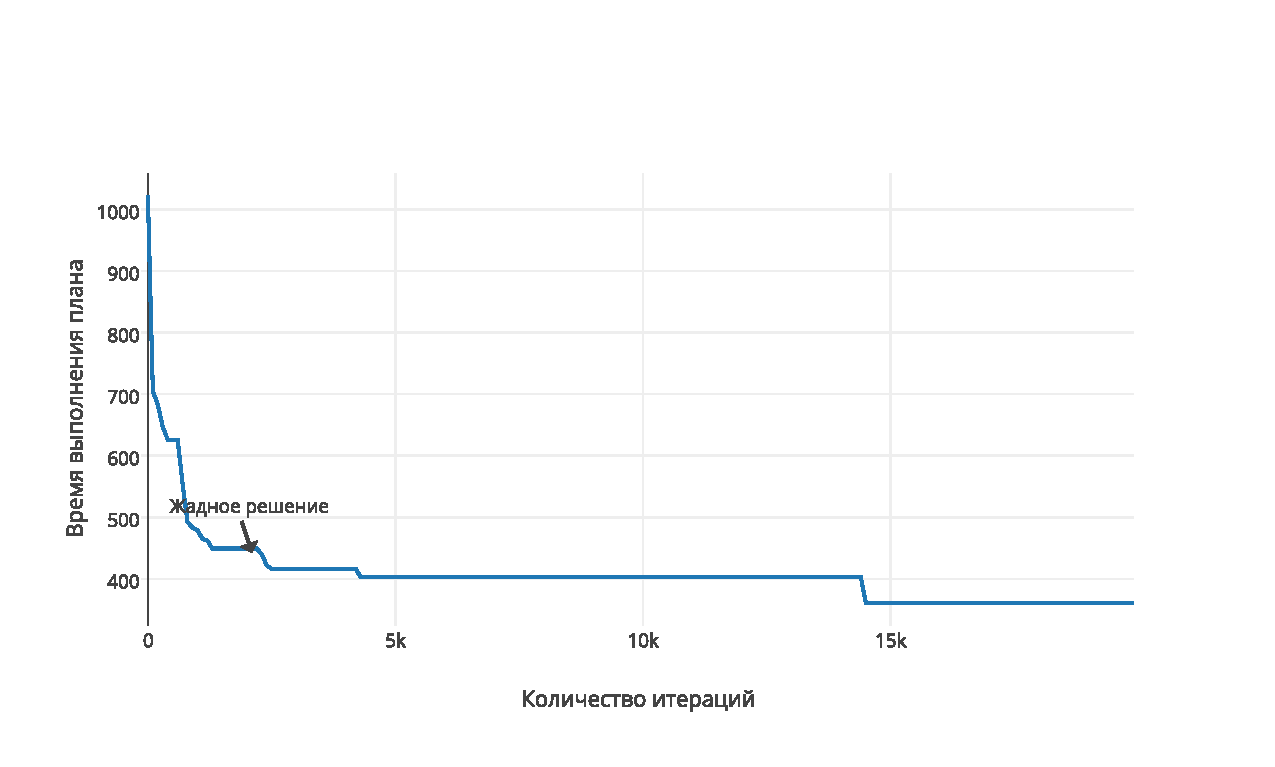
\includegraphics[scale=0.8]{images/iter-value-20-plot.eps}
\caption{Стоимость решения ГА в зависимости от количества итераций для 20 заданий}
\label{fig:iter-20}
\end{figure}


\begin{figure}[here]
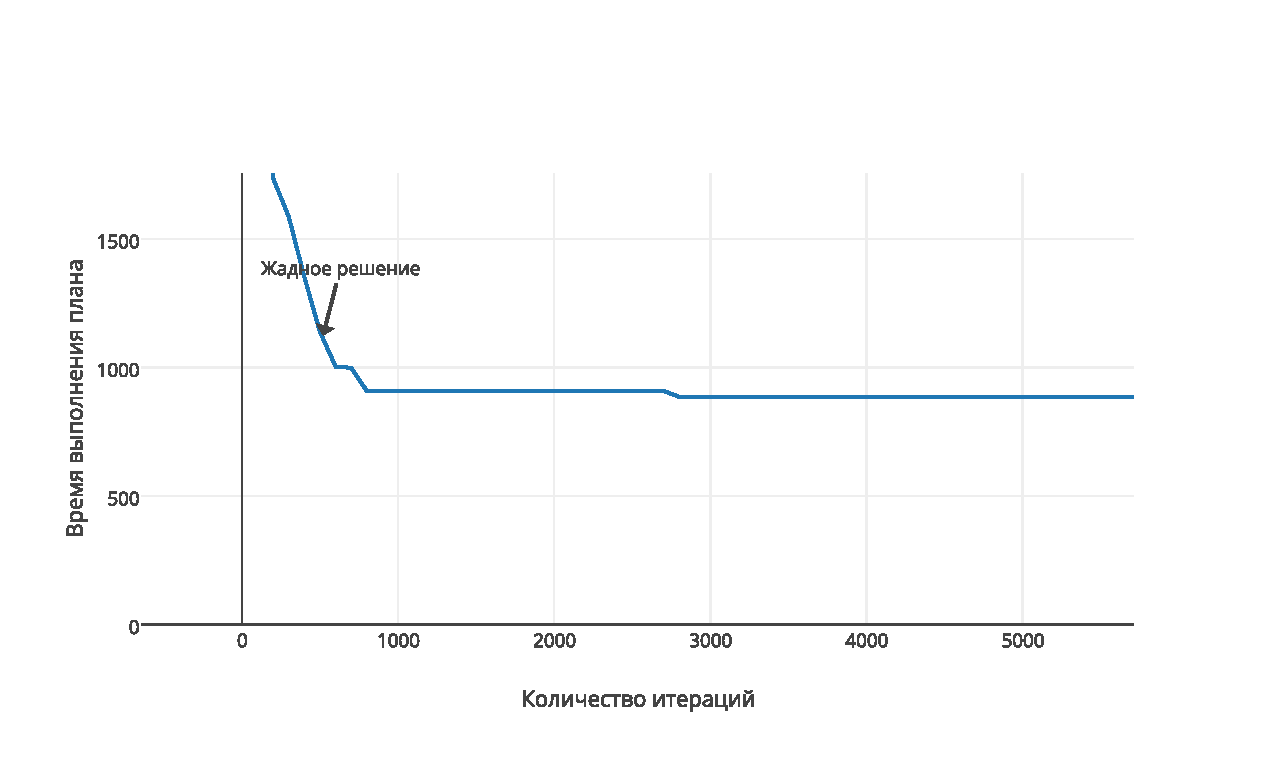
\includegraphics[scale=0.8]{images/iter-value-30-plot.eps}
\caption{Стоимость решения ГА в зависимости от количества итераций для 30 заданий}
\label{fig:iter-30}
\end{figure}
\pagebreak

На \cref{fig:iter-20} показан график стоимости решения в зависимости от количества итераций ГА. 5 тысяч итераций генетический алгоритм осуществляет примерно за 3-4 минуты. Здесь решение, полученное с помощью ГА на 50 единиц времени более быстрое чем, решение, полученное жадным алгоритмом, что составляет 25\%. Видно, что этот результат можно значительно улучшить, выполняя ГА на 10 минут дольше.

Также \cref{fig:iter-30} показывает, что ГА имеет смысл использовать на входных данных в 30 заданий.

\pagebreak
\begin{figure}[here]
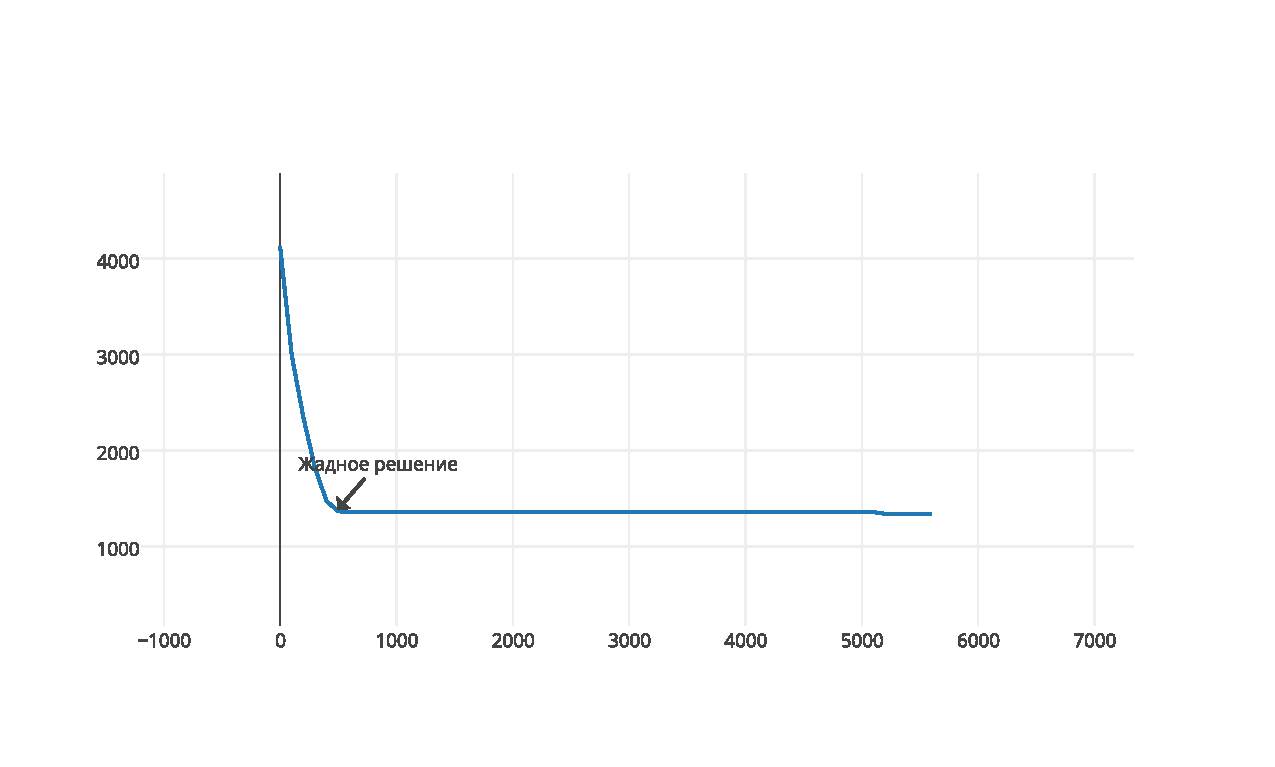
\includegraphics[scale=0.8]{images/iter-value-50.eps}
\caption{Стоимость решения ГА в зависимости от количества итераций для 40 заданий}
\label{fig:iter-40}
\end{figure}

На графике \cref{fig:iter-40} можно увидеть, что ГА не дает значительного прироста в точности решения для 40 заданий. С учетом того, что жадный алгоритм работает значительно быстрее, решено использовать именно его для входных данных от 40 заданий.

В результате всех экспериментов планировщик СПУ для подводных аппаратов работает в следующем режиме.
\begin{itemize}
\item Если количество заданий не превышает 18, запускается существующее точное решение.
\item При количестве заданий от 19 до 40 запускается генетический алгоритм.
\item Для остальных размеров входных данных задания распределяются с помощью жадного алгоритма.
\end{itemize}

\section{Заключение}
В процессе работы был реализован ряд алгоритмов, решающих задачу планирования заданий для группы АНПА в рамках модели \eqref{varm1}~--~\eqref{varm3}. Созданы программы, позволяющие оценить качество их работы. Некоторые из реализованных алгоритмов были внедрены в СПУ для автономных подводных аппаратов ДВФУ.

Был получен опыт в поиске и изучении научных статей, значительно улучшены знания в области генетических алгоритмов.

Тема работы имеет потенциал для дальнейшего развития. Для решения задачи следует рассмотреть другие эвристические подходы, а также методы децентрализованного управления группой аппаратов.

В рамках работы было написано 3000 строк кода на языках C++ и Python, 120кб.


\pagebreak

\bibliographystyle{ugost2008}
\bibliography{report}


\end{document}
